\documentclass[aip,jcp,reprint,a4paper,onecolumn,nofootinbib,amsmath,amssymb]{revtex4-1}
% Options for onecolumn and a4paper
\linespread{1.0}
\usepackage[expansion,protrusion,tracking=smallcaps]{microtype}
\usepackage{chemformula,tikz}
\usepackage{listings,xcolor}
\lstset{
  basicstyle = \small\ttfamily,
  keywordstyle = \color{blue!80!black},
  commentstyle = \color{green!40!black},
  columns = fullflexible,
  xleftmargin = 1em
}
\lstdefinelanguage{espresso}[]{TCL}{%
  morekeywords={part,reaction,minimize_energy},
  deletekeywords={range}
}
\lstnewenvironment{espresso}[1][]%
  {\lstset{language=espresso,#1}}%
  {}
\lstnewenvironment{bash}[1][]%
  {\lstset{keywordstyle = \color{red!80!blue},keywords={\$},#1}}%
  {}
\usepackage{xspace}
\newcommand\code{\lstinline}
\newcommand{\es}{\mbox{\textsf{ESPResSo}}\xspace}
\newcommand\codees{\lstinline[language=espresso]}
\renewcommand\thefootnote{\fnsymbol{footnote}}
\begin{document}
\title{Catalytic Reactions Tutorial}
\author{Henri Menke}
\email[]{\texttt{henri@icp.uni-stuttgart.de}}
\affiliation{Institute for Computational Physics,
  Universit\"at Stuttgart,
  Allmandring 3,
  D-70569 Stuttgart,
  Germany}
\author{Joost de Graaf}
\email[]{\texttt{jgraaf@icp.uni-stuttgart.de}}
\affiliation{Institute for Computational Physics,
  Universit\"at Stuttgart,
  Allmandring 3,
  D-70569 Stuttgart,
  Germany}
\affiliation{School of Physics and Astronomy,
  University of Edinburgh,
  Scotland, Edinburgh EH9 3JL,
  United Kingdom}
\date{\today}

\begin{abstract}
  In this tutorial we explore how to simulate catalytic reactions using \es\ for the purpose of modeling self-propelled particles (swimmers). We discuss the implemented reaction schemes and use one of them to study the enhanced translational diffusion of a catalytic swimmer. This should give a basic introduction on how to setup simulations involving catalytic reaction in \es\ and ideally enable you to conduct your own numerical experiments involving catalytic swimmers.
\end{abstract}

\maketitle

\section{Cataltic Reactions}

Many chemical processes in nature do not occur at room temperature, because the energy penalty is too high to be overcome by thermal fluctuations. The activation energy of such processes can in some cases be lowered significantly in the presence of a catalyzer (a catalytic substance). Below, we discuss this concept in some detail, in order to prepare you for its application to catalytic swimmers.

We may write a general equilibrium reaction as
\begin{equation}
  \label{eq:equi}
  \ch{!(reactants)(R) <=> !(products)(P)}
\end{equation}
where \ch{R} are the reactants and \ch{P} are the products. We restrict ourselves to the situation where there is a single product and single reactant in the following. The double headed arrow is used to indicate that this reaction is in an equilibrium. The equilibrium reation~\eqref{eq:equi} can be described by the equilbrium reaction constant
\begin{equation}
  \label{eq:const}
  K_{\text{eq}} = \frac{k_{\text{eq},+}}{k_{\text{eq},-}} = \frac{[\ch{P}]}{[\ch{R}]} ,
\end{equation}
with $[\ch{P}]$ and $[\ch{R}]$ the product and reactant concentration and $k_{\textrm{eq},\pm}$ the forward and backward reaction rates. The chief effect of the reaction is a change of the concentrations of reactants and products over time, whenever the system is brought out of equilibrium. It pushes the system to maintain a steady-state concentration ratio between the products and reactants, governed by the equilibrium contstant $K_{\text{eq}}$. The associated differential equations can be written as
\begin{subequations}
  \label{eq:diff}
  \begin{align}
    \label{eq:diff-equi-a}
    \frac{d[\ch{R}]}{dt} &= + k_{\text{eq},-}[\ch{P}] - k_{\text{eq},+}[\ch{R}] , \\
    \label{eq:diff-equi-b}
    \frac{d[\ch{P}]}{dt} &= - k_{\text{eq},-}[\ch{P}] + k_{\text{eq},+}[\ch{R}] .
  \end{align}
\end{subequations}

A catalyzer shifts the free energy landscape in favour of one of the constituents \ch{R} or \ch{P}. We choose \ch{P}, since it stands for the products and we want to enhance the forward reaction.
\begin{equation}
  \ch{!(reactants)(R) <=>>[ !(catalyzers)(C) ] !(products)(P)} .
\end{equation}
If the back reaction rate is very small by comparison, it can be ignored and effectively the reaction only occurs in one direction.
\begin{equation}
  \label{eq:cat}
  \ch{!(reactants)(R) ->[ !(catalyzers)(C) ] !(products)(P)} .
\end{equation}
In the case of excessive catalysis~\eqref{eq:cat} the back reaction rate $k_{\text{eq},-}$ can be set to zero and the forward reaction rate is enhanced $k_{\text{eq},+} \to k_{\text{ct}}$. The rate equations~\eqref{eq:diff} then reduce to
\begin{equation}
  \label{eq:diff-cat}
  -\frac{d[\ch{R}]}{dt} = \frac{d[\ch{P}]}{dt} = k_{\text{ct}}[\ch{R}] ,
\end{equation}
which has a simple exponential solution $R(t) = R(0)\exp(- k_{\text{ct}} t)$ and $P(t) = P(0) + R(0)(1 - \exp(- k_{\text{ct}} t))$.

What we have discussed so far is a continuum model, as no actual particles are involved in the picture, only concentrations. To simulate such a simple catalytic reaction with molecular dynamics we need to come up with a minimal model. Phenomenologically, catalysis is triggered by a contact interaction,~\emph{i.e.}, the reactant has to make physical contact with the catalyzer. \es\ technically only simulates point particles --- they obtain a size through the interaction potentials. To impose a finite extent, we define a \emph{reaction range} around the catalyzer inside of which the conversion of a reactant to a product is feasible. This means that we have explicit catalyzer, reactant, and product particles, for which the inter-particle distance imposes whether a reaction takes place or not.

Next we have to think about how to implement \eqref{eq:diff-cat} is this picture. Simply integration \eqref{eq:diff-cat} yields an exponential decay as a function of time, see above. The reaction move is a stochastic process and takes place with a certain probability, depending on the reaction rate. This probability is inversely proportional to the exponential decay. We assign
\begin{equation}
  \label{eq:prob}
  P_{\text{move}} = 1 - \mathrm{e}^{-k\,\Delta t} ,
\end{equation}
with the reaction rate $k \in \{ k_{\text{eq},+}, k_{\text{eq},-}, k_{\text{ct}} \}$ and the simulation time step $\Delta t$.

\section{Cataltic Reactions in \es}

There are two implementations of the reaction scheme~\eqref{eq:diff-equi-a},~\eqref{eq:diff-equi-b}, and~\eqref{eq:diff-cat}, which we will refer to as \emph{number conserving} and \emph{non-number-conserving}. In the following we will discuss both of these schemes in detail. In all cases, there are only three species of the $N \ge 3$ possible species you can define in \es\ involved in the catalytic reaction. Multiple reactions involving a variety of species are not possible at this moment.

\subsection{Non-Number-Conserving Scheme}

In \es\ we assume the equilibrium constants in equations~\eqref{eq:diff} to be equal,~\emph{i.e.}, $k_{\text{eq},+} = k_{\text{eq},-}$. Thus, according to~\eqref{eq:const}, the reaction constant $K = 1$. The equilibrium constant is applied the reactant and product particles in the system and determines the conversion rate between these two. Essentially, this ensures that when there is a catalytic reaction, the fuel does not run out and the system is essentially coupled to a `chemical bath'. For reactants in the vicinity of the catalyzer (as determined by the \emph{reaction range}) the forward reaction is favoured and no back conversion will take place there. Also the forward reaction rate is enhanced to $k_{\text{ct}}$ and can be specified as an input parameter. The catalyzer particles drive the system out of equilibrium.

\begin{figure}
  \centering
  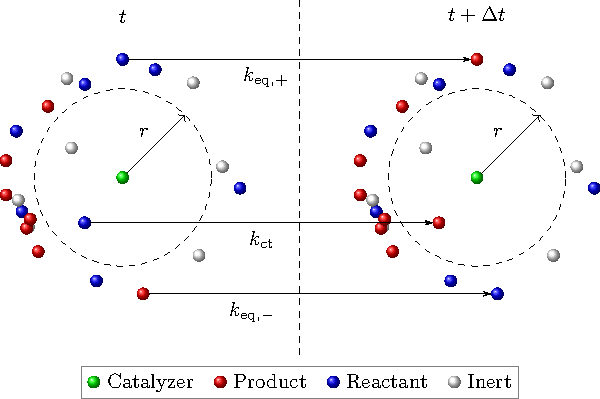
\includegraphics{FIGURES/non-number-conserving}
  \caption{\label{fig:nnc}Illustration of the \emph{non-number-conserving} scheme. Within a cut-off radius $r$ of the catalyzer (green), the reactant particles (blue) can be converted into products (red); inert particles (white) are left unaffected by the reactions taking place. The catalytic conversion is indicated using the arrow labeled $k_{\text{ct}}$, which shows the result of a conversion event taking place in one time step $\Delta t$ (from left panel to right panel). Outside of this region a homogeneous equilibrium reaction takes place, that pushes the out-of-equilibrium concentrations produced by the catalyzer back towards equilibrium. This is indicated by the two arrows which cause conversion of products into reactants with $k_{\text{eq},-}$ and reactants into products with $k_{\text{eq},+}$. Even though $k_{\text{eq},+} = k_{\text{eq},-} = k_{\text{eq}}$ in \es, we show them seperately to emphasise that one is a forward and one is a back reaction.}
\end{figure}

Figure~\ref{fig:nnc} shows the reaction scheme explained before pictorially. Within the reaction range, determined by $r$, the equilibrium reactions are also allowed to take place, but additionally the forward reaction is catalysed. Within one time step bulk reactions take place with the equilibrium constant. These might occur in both directions and push the the out-of-equilibrium concentrations produced by the catalyzer back towards the steady state. It is clear that it does not make sense to set $k_{\text{eq}} > k_{\text{ct}}$, as this would shadow the effect of the catalyzer compared to that of the equilibrium reactions in bulk.

The sketch in figure~\ref{fig:nnc} and the above discussion explain why the scheme is called \emph{non-number-conserving}. Namely, the number of products and reactants is not constant over time, even in the steady state there are short-time fluctuations. However, the overall number of particles is conserved. This is representative of the physical reality of a catalytic reaction, but frustrates the use of this algorithm in a number of situations. If, for instance, any of the species swapped around are charged, then the total charge of the simulation box need not be conserved, and by extention, the box need not be charge neutral. The electrostatic algorithms in \es\ break down for non-neutral boxes. In order to allow for the use of electrostatic algorithms, we introduce the \emph{number-conserving} scheme next.

\subsection{Number-Conserving Scheme}

In this scheme, we disallow bulk reactions of single particles\footnote{One can set the equilibrium reaction rate $k_{\text{eq}} = 0$ to achieve this as well.} and allow a reaction inside the reaction range involving only rectant-product pairs. Simply exchanging the particles in the pair would not yield an effect, when averaged over time, since the exchange occurs isotropically. We therefore introduced an additional symmetry breaking, namely of the spatial coordinate. This also conveniently allows us to model catalytic Janus swimmers.

\begin{figure}
  \centering
  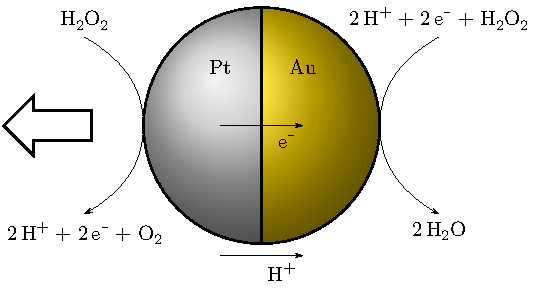
\includegraphics{FIGURES/janus-particle}
  \caption{\label{fig:janus}A Janus swimmer, having a catalytic surface on both hemispheres, may support two different (redox) reactions. This results in breaking of reflection symmetry which propels the particle in the direction of the large arrow.}
\end{figure}

Consider such a swimmer, see Fig.~\ref{fig:janus}, consisting of \ch{Pt} on one hemisphere and \ch{Au} on the other hemisphere. Both surfaces enhance a reaction, here~\cite{Gibbs_10,Wheat_10}
\begin{align}
  \label{eq:H2O2}
  \ch{
    H2O2 &->[ Pt ] 2 H^+ + 2 e^- + O2 \\
    2 H^+ + 2 e^- + H2O2 &->[ Au ] 2 H2O
  }
\end{align}
The block arrow in the sketch points in the direction of movement induced by the reaction. We refer to upper and lower hemisphere (or half-space) in the following, as two regions that are determined with respect to the orientation of the particle and the plane through the center of the particle, with the orientation as its normal. In the present case one might choose \ch{Au} as the upper hemisphere and \ch{Pt} as the lower hemisphere. The reaction region is, as before, bounded by the \emph{reaction range} $r$.

\begin{figure}
  \centering
  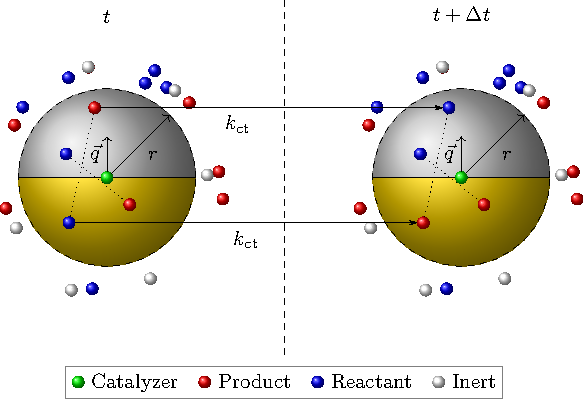
\includegraphics{FIGURES/number-conserving}
  \caption{\label{fig:nc}Illustration of the \emph{number-conserving} scheme. The cut-off range of $r$ around the catalyzer (green) is subdivided into two half-spaces in analogy to figure~\ref{fig:janus}. A reactant-product pair (blue and red connected by dotted line)is converted by swapping them if the pair is selected, and only if the product (red) resides in the upper half-space (silver background) and the corresponding reactant (blue) resides in the lower half-space (gold background). The catalytic reaction leads to a conversion of one reactant-product pair of particles in this example, denoted by the arrows annotated with $k_{\text{ct}}$. The second reactant-product pair within the reaction range is not viable for conversion. Additionally, particles in a pair may only undergo one exhange per time step.}
\end{figure}

For simplicity, in the simulation we abstract away all the reaction mechanism including the electron transport through the Janus particle. The proton transport around the particle (through, diffusion, advection, and migration) is taken into account implictily via the thermalized MD simulation. We end up with a simple scheme,
depicted in figure~\ref{fig:nc}.

As already explained, reactions can only take place for reactant-product pairs. The conversion is such that a reactant is converted to a product and a product is converted to a reactant. This ensures conservation of the particle number for each type. To model a Janus particle as in Fig.~\ref{fig:janus}, we allow an exchange move only when the following conditions are met:
\begin{enumerate}
\item Both partners of the reactant-product pair have to reside within
  the reaction range.
\item The product has to reside in the upper half-space of the
  reaction range.
\item The reactant has to reside in the lower half-space of the
  reaction range.
\end{enumerate}
This is illustrated in Fig.~\ref{fig:nc}.

\subsection{Usage in \es}

Catalytic reactions can be enabled in \es\ by compiling in the eponymous feature \code{CATALYTIC_REACTIONS}. The number-conserving method additionally requires the \code{ROTATION} feature to provide the particles with an orientation vector. In \es\ the orientation of the particle is defined by a quaternion; this in turn defines a rotation matrix that acts on the particle's initial orientation (along the $z$-axis), which then defines the particles current orientation~\cite{UG,Limbach_06,Arnold_13}.

In \es\ particles are set up using the \codees{part} command. It allows to set various options, such as the initial position (mandatory), the type, and the charge. To setup the reaction there is the \es\ command \codees{reaction}, which operates on particle types. The general syntax is
\begin{espresso}
reaction reactant_type R catalyzer_type C product_type P range r ct_rate k_ct
    [eq_rate k_eq] [react_once on/off] [swap on/off]
\end{espresso}
The parameters in square brackets are optional and can be left out. They will then assume their default values which are \codees{eq_rate 0.0}, \codees{react_once off}, and \codees{swap off}.

\noindent\textbf{Important:} Due to the method of implementation there can only be one reaction. You can alter the reaction parameters, but you may not change the reaction partners.

To set up a reaction between the types 1 and 2, where particles of type 3 act as catalyzers with a reaction range of 1.5 around them with a reaction rate of 20, one types
\begin{espresso}
reaction reactant_type 1 catalyzer_type 3 product_type 2 range 1.5 ct_rate 20
\end{espresso}
Here we have left out the optional parameters, but their meaning is nevertheless important. The first one, \codees{eq_rate}, should be self explanatory; it sets the equilibrium reaction rate as detailed in the introductory sections. The \codees{react_once} parameter determines whether a particle can take part in a only single reaction move per time step. In the case of multiple catalyzers in the system a particle might be tagged for reaction several times by different catalyzers because their reaction ranges overlap and the reactant is inside this overlap. This can be  prevented by setting \code{react_once on}. That way the reaction rate is independent of the density of catalyzers. This can be convenient if one wants to model a surface using several catalyzer particles that are in close proximity to one another, but still have a uniform catalytic conversion rate for the entire surface. Finally, the parameter \codees{swap} determines which scheme to use; \codees{swap off} uses the not number conserving scheme, \codees{swap on} uses the number-conserving scheme. The name `swap' originates from the sketch figure~\ref{fig:nc}, because it looks as if the particles are swapped.

However, the \codees{swap} option does not really swap the particles, but only exchanges their type (and their charge, if \es\ was compiled with \code{ELECTROSTATICS}). This means that the particle numbers do not change. This allows one to track how frequently a particle undergoes a reaction, by tracking the properties of a particle via the particle number.

\section{Configuring \es\ for Catalytic Reactions}

For this tutorial to work you need a version of \es\ containing the catalytic reactions feature with the \codees{swap} mechanism. Therefore check out the \es\ online repository at \url{https://github.com/espressomd/espresso}. If you have installed \code{git}, you can issue on the command line
\begin{bash}
$ git clone https://github.com/espressomd/espresso.git
\end{bash}
Now you are ready to build \es. Change to the newly created directory and use the following commands to configure \es\ for compilation.
\begin{bash}
$ mkdir build
$ cd build
$ cmake ..
\end{bash}
After this, you will need to copy the \code{myconfig-sample.hpp} file into \code{myconfig.hpp} and select the appropriate \code{FEATURES} in the latter.
\begin{bash}
$ cp myconfig-sample.hpp myconfig.hpp
\end{bash}
To run all the tutorials you need to uncomment the following \code{FEATURES}:
\begin{lstlisting}[language=c]
#define ROTATION
#define ROTATIONAL_INERTIA
#define LANGEVIN_PER_PARTICLE
#define CATALYTIC_REACTIONS
#define LENNARD_JONES
\end{lstlisting}
Now you are ready to build \es.
\begin{bash}
$ make -j N
\end{bash}
with $N$ the number of processes used to build. Next you can unpack the archive with the tutorial files in this directory. You will find two folders, one called `EXERCISES' and one called `SOLUTIONS'.


\section{The Enhanced-Diffusion Tutorial}

In the folder `EXERCISES' you will find the \code{reaction.tcl} file. It is a tutorial to demonstrate that our approach to catalytic reactions leads to enhanced diffusion of the catalyzer. When you begin, the code is incomplete and will produce errors when evaluated in \es. It needs your input to function properly. A fully functional file exists in the `SOLUTIONS' folder, but we recommend that you try solving the exercises on your own first.

To start the exercises, go into the `EXERCISES' directory and invoke \es\ on the script
\begin{bash}
$ ./../build/Espresso reaction.tcl 0
\end{bash}
where the parameter \code{0} determines whether the reaction is enabled. Here, 0/1 corresponds to reaction off/on, just like on your VCR. At this stage, executing the above line will cause an error, as the exercise has not yet been completed.

\subsection{Structure of the Simulation}

Let's walk through the script. It is best to open the file while reading this.

First, we read the activity parameter from the command line and verify it. Then we set up some general simulation parameters, such as box length, radius of the colloid, concentration of reactant and products, and the reaction rate. Next, we setup the thermostat parameters, but do not enable it yet.

Before we can set up the colloid and the small particles around, the first two exercises have to be completed.

The script continues to setup interactions between the colloid and the smaller particles and, most importantly, the reaction. The syntax for setting up a reaction is given above in the section ``Usage in \es''.

Warmup is performed by the \codees{minimize_energy} routine. It has several advantages over traditional force-capping warmup, which you will learn about when completing the associated exercise.

Now the thermostat is enabled and the equilibration is performed. Finally, we perform five production runs in which we measure the mean-square displacement (MSD) and the angular velocity auto-correlation function (AVACF).

You should have learned about everything that does not have to with catalytic reactions in previous tutorials. If you are unfamiliar with any concept, it might be better to go back and complete the other tutorials first.

\subsection{What to Expect}

Once you have completed all the tasks in the exercise script, the time has come to run the actual simulation. Run the script twice, once with the activity parameter set to 0 and once set to 1. You will have two directories: \code{active-system} and \code{passive-system}. These contain MSD and AVACF data files numbered consecutively over the
different runs.

It is now your job to average over these five files. You can do this in \code{gnuplot} or the scripting language of your choice. The MSD files have five columns each. The first two columns are time and samples, the last three are $x$, $y$, $z$. The AVACF files have only three columns, where the first two are also time and samples and the
third is the AVACF averaged over all spatial components. For the MSD we still have to average over the three spatial dimensions.

When we have extracted the mean (and recommendably the standard error) we can plot it over time to achieve plots as in Figs.~\ref{fig:msd} and~\ref{fig:avacf}. We can clearly see, that the reaction facilitates enhanced translational diffusion while
leaving the rotational diffusion unaffected.

\begin{figure}[tb]
  \centering
  \leavevmode\hfill
  \begin{minipage}[t]{.45\linewidth}
    \centering
    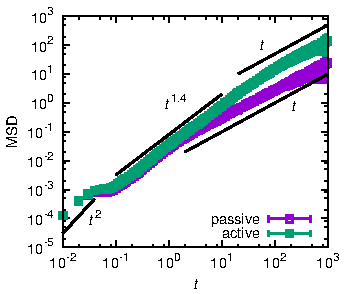
\includegraphics{FIGURES/msd}
    \caption{Averaged MSD over five runs with standard error on the
      error bars for both, the active and the passive system. The
      black lines serve as a guide to the eye and indicate the
      dependence of the MSD on the time $t$.}
    \label{fig:msd}
  \end{minipage}
  \hfill
  \begin{minipage}[t]{.45\linewidth}
    \centering
    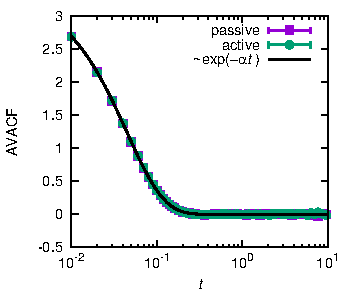
\includegraphics{FIGURES/avacf}
    \caption{The AVACF for the same system as in
      figure~\ref{fig:msd}. Note that the activity does not influence
      the rotational behavior.}
    \label{fig:avacf}
  \end{minipage}
  \hfill\null
\end{figure}

Specifically, a passive particle shows a $t^{2}$ ballistic regime, typical for Langevin type simulations, followed by an intermediate regime, where the slope changes gradually to the long-time diffusive $t$. The active swimmer, shows similar behavior. However, the intermediate regime is stretched, with the long-time diffusion setting in only at around $t = 10$ (which corresponds to one rotational diffusion time). This is because the self-propulsion induces a persistent motion along the particle axis, leading to a more-or-less $t^{2}$ MSD; here a little less as the increase matches $t^{1.4}$ better. The only thing that breaks this persistence is rotational diffusion. Hence beyond a time for which the orientation of the particle randomizes, the behavior becomes diffusive again, albeit with a higher diffusion coefficient. It is therefore important to show that the rotational diffusion remains unaffected by the particle catalyzing solutes in its surrounding.

\section{Concluding Remarks}

With that, you have come to the end of this tutorial. We hope you found it informative and that you have a sufficient understanding of the way to deal with catalytic reactions in \es\ to set up simulations on your own.

\section*{References}

\bibliographystyle{unsrt}
\bibliography{refs}

\end{document}

%%% Local Variables: 
%%% mode: latex
%%% End:
